\documentclass[12pt,a4paper,twoside]{article}
\usepackage[utf8]{inputenc}
\usepackage{amsmath}
\usepackage{lmodern}
\usepackage{textcomp}
\usepackage{amsfonts}
\usepackage{amssymb}
\usepackage{graphicx}
\usepackage[left=2cm,right=2cm,top=2cm,bottom=2cm]{geometry}
\author{Cabello Lopez Marco Antonio\\
Actividad 5\\
Departamento de Fisica\\
Universidad de Sonora}
\date{Hermosillo, Sonora a Lunes 13 de Noviembre del 2017}
% used in maketitle                                                             
\title{\textbf{Movimiento de Traslacion}}
\begin{document}
\maketitle
\section{Planteamiento del problema}
En esta actividad se pide calcular algunos parametros del movimiento de traslacion de nuestro planeta, apoyados con Fortran.

Apoyandonos con las notas del movimiento circular uniforme.

\begin{figure}[h!]
  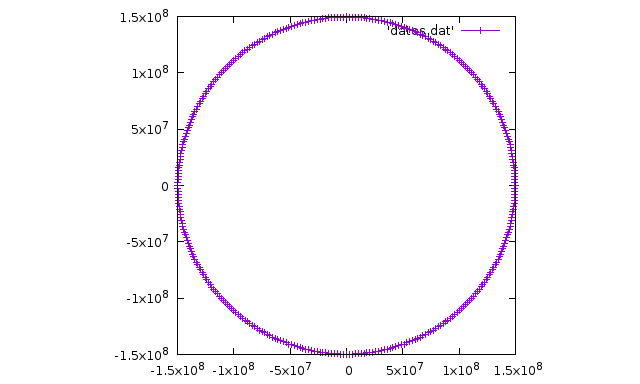
\includegraphics[width=\linewidth]{movt.png}
  \caption{Grafica de posiciones}
  \label{fig:Grafica}
\end{figure}

\begin{document}
\maketitle
\section{Traslación de la Tierra}
La traslación es el movimiento en el cual la Tierra orbita alrededor del Sol. La distancia promedio entre estos cuerpos es de 149,600,000 kilometros, tomando por lo tanto un tiempo total de 365.256 dias en completar su orbita el planeta Tierra.

\section{Calculo de posición}
Es posible calcular la posición de la Tierra alrededor del sol utilizando coordenadas y dando el angulo al cual queremos encontrar su posición. Donde r es la distancia entre la Tierra y el sol.
\begin{equation}
x= r * \cos\theta
\end{equation}
\begin{equation}
y= r * \sin\theta
\end{equation}

\clearpage
\section{Codigo del programa}
\begin{verbatim}
FUNCTION fx(g) RESULT (x)
	double precision, intent(IN) :: g
	double precision 	     :: x
	 x = 1.496d8 * dcos(g)
END FUNCTION fx

FUNCTION fy(g) RESULT (y)
	double precision, intent(IN) :: g
	double precision 	     :: y
	 y = 1.496d8 * dsin(g)
END FUNCTION fy

PROGRAM movt

	IMPLICIT NONE
	integer :: i
	double precision :: g, fx, fy
	double precision, parameter :: r = 1.496d8, pi=3.1416d0 !KILOMETROS
	double precision, dimension(1000) :: x, y

 
OPEN (1, FILE = 'datos.dat', STATUS = 'unknown')
 DO i=1, 360, 1
 g = dble(i)
 g = g * pi / 180.0d0
 x(i) = fx(g)
 y(i) = fy(g)
 WRITE (1,*) x(i), y(i)
 WRITE (1,*) ' '
 END DO
 CLOSE (1)


END PROGRAM movt
\end{verbatim}




\end{document}